\documentclass{beamer}
\usepackage{ctex, hyperref}
\usepackage[T1]{fontenc}

% other packages
\usepackage{latexsym,amsmath,xcolor,multicol,booktabs,calligra}
\usepackage{graphicx,pstricks,listings,stackengine}
\usepackage{caption}
\usepackage{multicol}
\usepackage{wrapfig}
\usepackage{color}


\title{基于多源空间数据的广州市餐饮业选址}
\subtitle{本科毕业论文答辩}
\author{答辩人: 钟沛 \\ 指导老师: 陈艳男}
\institute{华南师范大学数学科学学院}
\date{2023年5月11日}
\usepackage{JilinUniv}

% defs
\def\cmd#1{\texttt{\color{red}\footnotesize $\backslash$#1}}
\def\env#1{\texttt{\color{blue}\footnotesize #1}}
\definecolor{deepblue}{rgb}{0,0,0.5}
\definecolor{deepred}{rgb}{0.6,0,0}
\definecolor{deepgreen}{rgb}{0,0.5,0}
\definecolor{halfgray}{gray}{0.55}

\lstset{
    basicstyle=\ttfamily\small,
    keywordstyle=\bfseries\color{deepblue},
    emphstyle=\ttfamily\color{deepred},    % Custom highlighting style
    stringstyle=\color{deepgreen},
    numbers=left,
    numberstyle=\small\color{halfgray},
    rulesepcolor=\color{red!20!green!20!blue!20},
    frame=shadowbox,
}


\begin{document}

\kaishu
\begin{frame}
    \titlepage
    \begin{figure}[htpb]
        \begin{center}
            
\includegraphics[width=0.15\linewidth]{pic/scnulogo.eps}
        \end{center}
    \end{figure}
\end{frame}

\begin{frame}
    \tableofcontents[sectionstyle=show,subsectionstyle=show/shaded/hide,subsubsectionstyle=show/shaded/hide]
\end{frame}


\section{选题背景及意义}
\begin{frame}{选题背景及意义}
    % \begin{itemize}[<+-| alert@+>] % 当然,除了alert,手动在里面插 \pause 也行
    \begin{itemize}
        \item 随着国内餐饮行业市场规模的不断扩大,餐饮行业的竞争也变得更加激烈,门店选址的重要性日益凸显\pause
        \item 选址要考虑的因素日益复杂,传统的选址方法不再受用,需要发掘更多基于大数据的选址方法\pause
        \item 当今基于大数据的选址模型
            \begin{itemize}
                \item 移动信令数据、GPS数据————在现实生活较难获取
                \item 有监督机器学习算法————容易受到数据标签的影响
            \end{itemize}
        % \item GitHub项目地址位于 \url{https://github.com/GohUnTsuan/JLU-Beamer-Theme},如果有bug或者feature request可以去里面提issue
    \end{itemize}\pause
    本文提出一种基于开源数据,将传统评价算法和机器学习算法结合的门店选址模型,为餐饮企业提供选址建议
\end{frame}


    



% \section{研究现状}

% % \subsection{Beamer主题分类}

% \begin{frame}{研究现状}
%     \begin{itemize}
%         \item 数据挖掘算法
%             \begin{itemize}
%                 \item 有监督学习方法
%                 \item 协同训练的半监督学习方法
%             \end{itemize}
%         \item 开源数据
%             \begin{itemize}
%                 \item POI数据
%                 \item 路网数据
%             \end{itemize}
%     \end{itemize}
% \end{frame}




% \section{研究思路}
% \captionsetup[figure]{labelformat=empty}
% \begin{frame}{研究思路}
%     \begin{figure}[htpb]
%         \centering
%         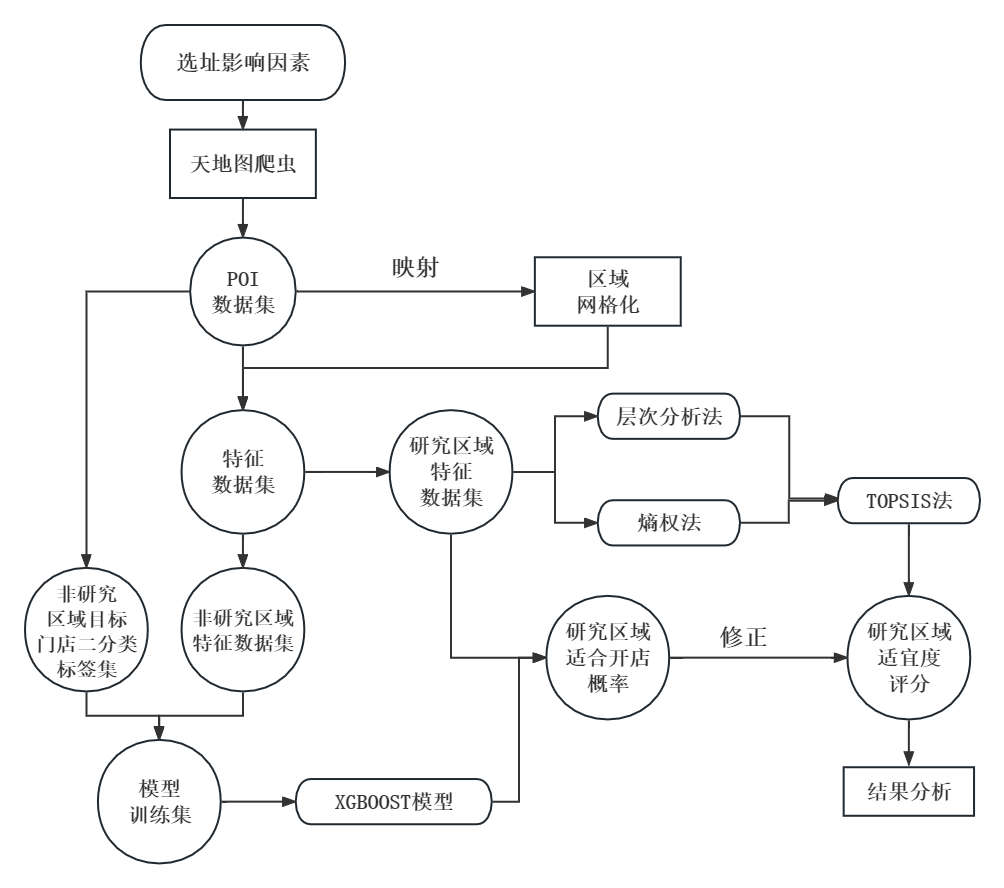
\includegraphics[width=0.75\linewidth]{pic/flow_chart.png}
%         % \caption{这个校徽就是矢量图}
%         \caption*{}
%     \end{figure}
% \end{frame}

\section{研究思路}
% \captionsetup[figure]{labelformat=empty}
\begin{frame}{研究思路}
    \begin{itemize}
        \item 研究区域\\
        {\textcolor[RGB]{255,0,0}{广州市天河区}}
        \item 目标选址门店 \\
        {\textcolor[RGB]{255,0,0}{冷饮店}}
        \item 选址分析 \\
        {\textcolor[RGB]{255,0,0}{借助适宜度评分}}
    \end{itemize}

\end{frame}
%     \begin{minipage}{0.45\textwidth}
%         % 左侧内容
%         \centering
%         {\large 研究区域}\\
%         {\textcolor[RGB]{255,0,0}{广州市天河区}}
%       \end{minipage}
%       \hfill
%       \begin{minipage}{0.45\textwidth}
%         \centering
%         {\large 目标选址门店}\\
%         {\textcolor[RGB]{255,0,0}{冷饮店}}

%       \end{minipage}
% \end{frame}

\begin{frame}{研究思路}   
    \begin{minipage}{0.37\textwidth}
        % 左侧内容
        影响因素
        \begin{itemize}
            \item 人口因素
                \begin{itemize}
                    \item 潜在消费者密度
                    \item 人口密度
                \end{itemize}
            \item 交通因素
            \begin{itemize}
                \item 交通流量
            \end{itemize}
            \item 竞争因素
            \begin{itemize}
                \item 竞争强度
            \end{itemize}
        \end{itemize}
        
      \end{minipage}
      \hfill
      \begin{minipage}{0.6\textwidth}
        % 插入图片
        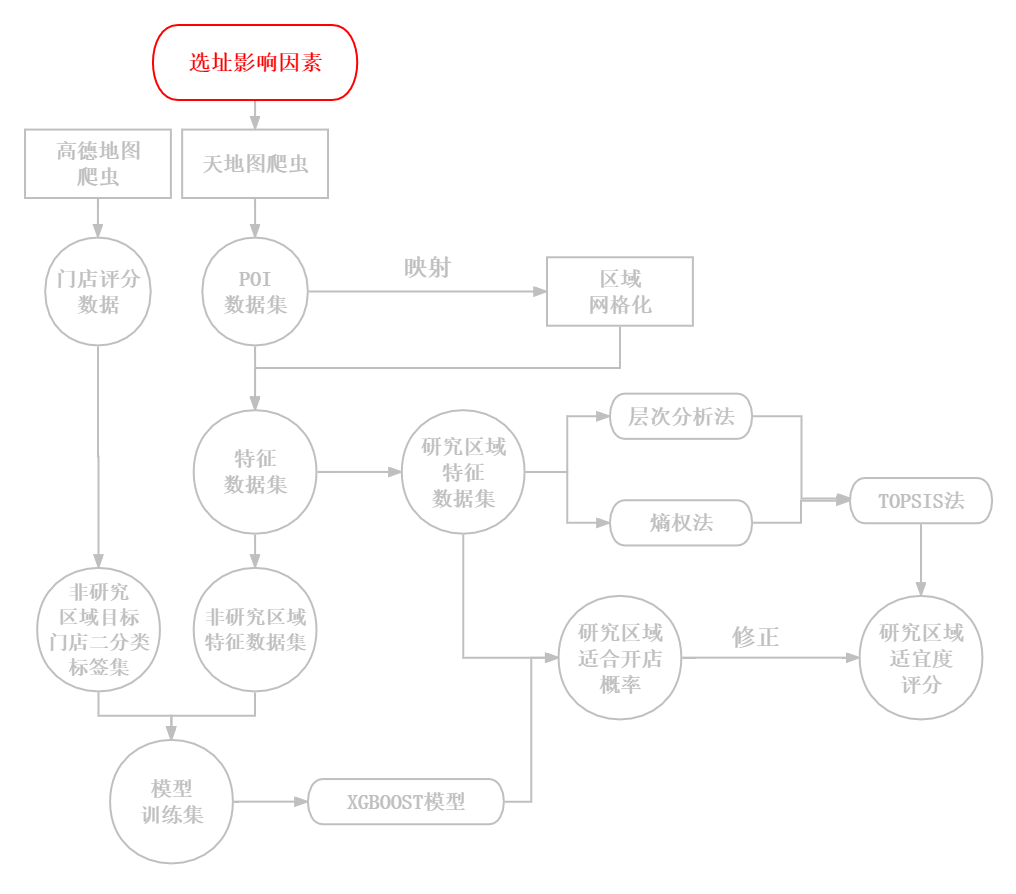
\includegraphics[width=1\textwidth]{pic/1.png}
      \end{minipage}
\end{frame}

\begin{frame}{研究思路}   
    \begin{minipage}{0.37\textwidth}
        % 左侧内容
        影响因素衡量
        \begin{itemize}
            \item 潜在消费者密度 \\
                {\footnotesize(商城、商务中心、中餐馆、快餐店)}
            \item 人口密度 \\
                {\footnotesize(大厦、小区、学校)}
            \item 交通流量 \\
                {\footnotesize(交叉路口、地铁站)}
            \item 竞争强度 \\
            {\footnotesize(冷饮店、咖啡店、酒吧)}
        \end{itemize}
        
        
      \end{minipage}
      \hfill
      \begin{minipage}{0.6\textwidth}
        % 插入图片
        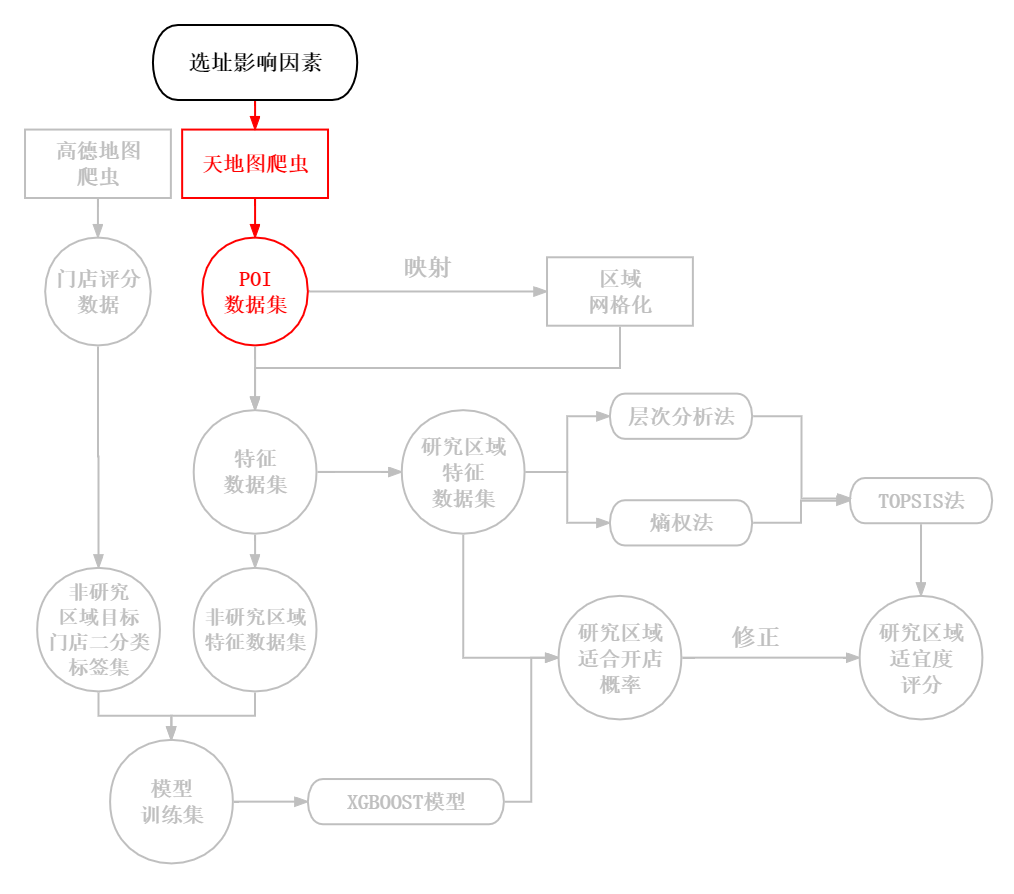
\includegraphics[width=1\textwidth]{pic/2.png}
      \end{minipage}
\end{frame}

\begin{frame}{研究思路}   
    \begin{minipage}{0.37\textwidth}
        % 左侧内容
        数据预处理
        \begin{enumerate}
            \item 地理图层网格划分 \\
            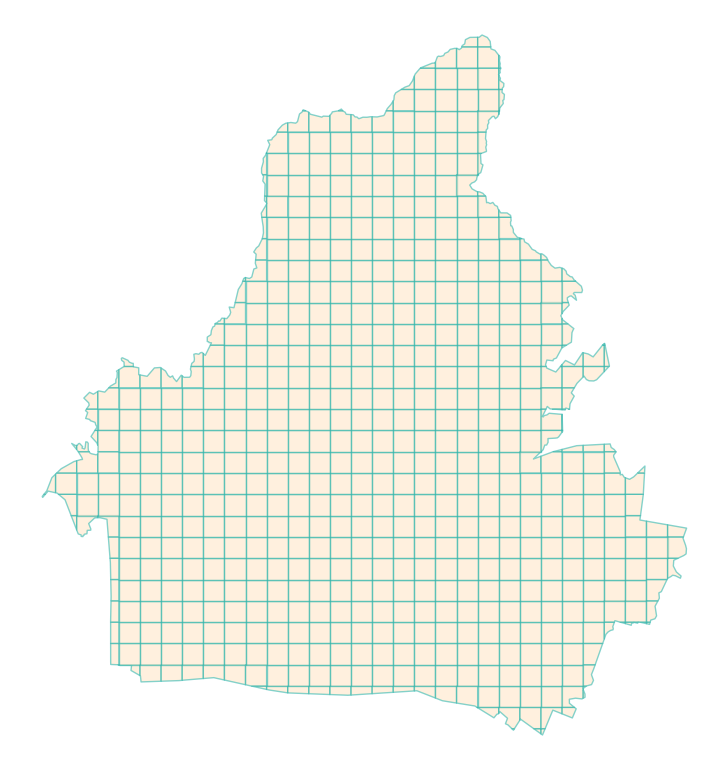
\includegraphics[width=0.5\textwidth]{pic/tianhegrid.png}
            \item 进行经纬度数据映射得到特征数据集
            
        \end{enumerate}
  
      \end{minipage}
      \hfill
      \begin{minipage}{0.6\textwidth}
        % 插入图片
        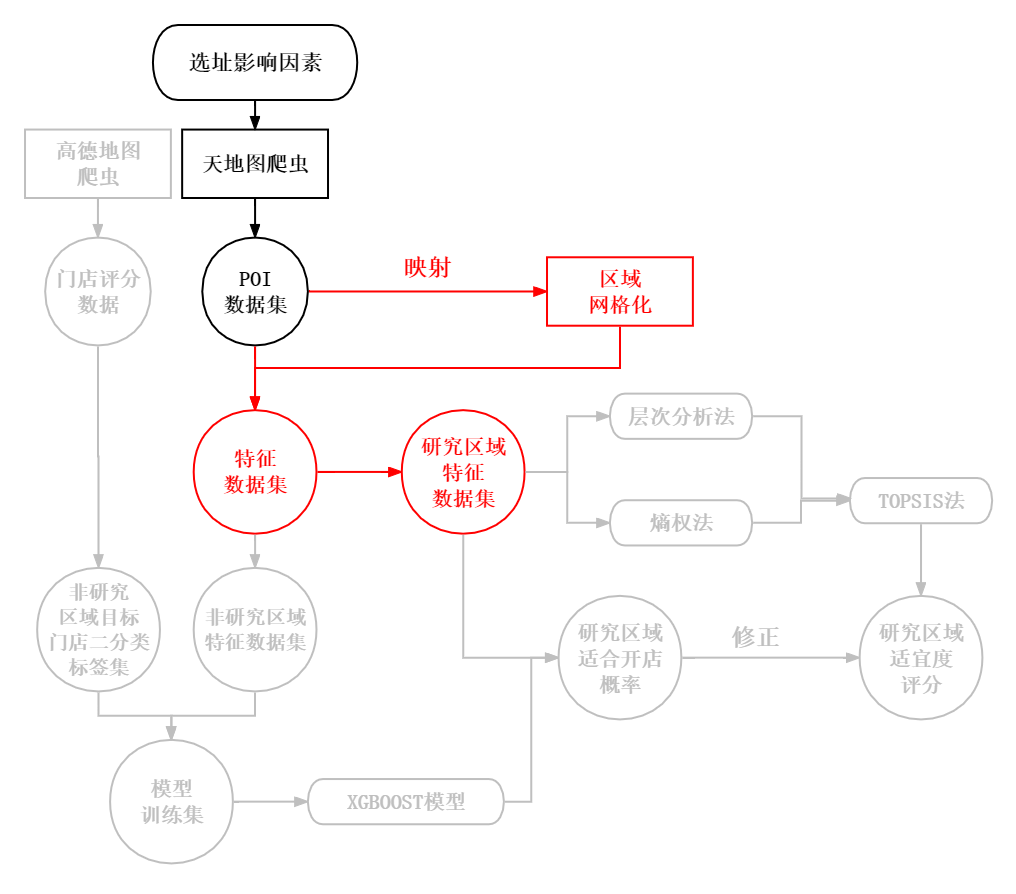
\includegraphics[width=1\textwidth]{pic/3.png}
      \end{minipage}
\end{frame}

\begin{frame}{研究思路}   
    \begin{minipage}{0.37\textwidth}
        % 左侧内容
        适宜度评分计算
        \begin{itemize}
            \item 层次分析法
            \item 熵权法
            \item TOPSIS法 
        \end{itemize}
  
      \end{minipage}
      \hfill
      \begin{minipage}{0.6\textwidth}
        % 插入图片
        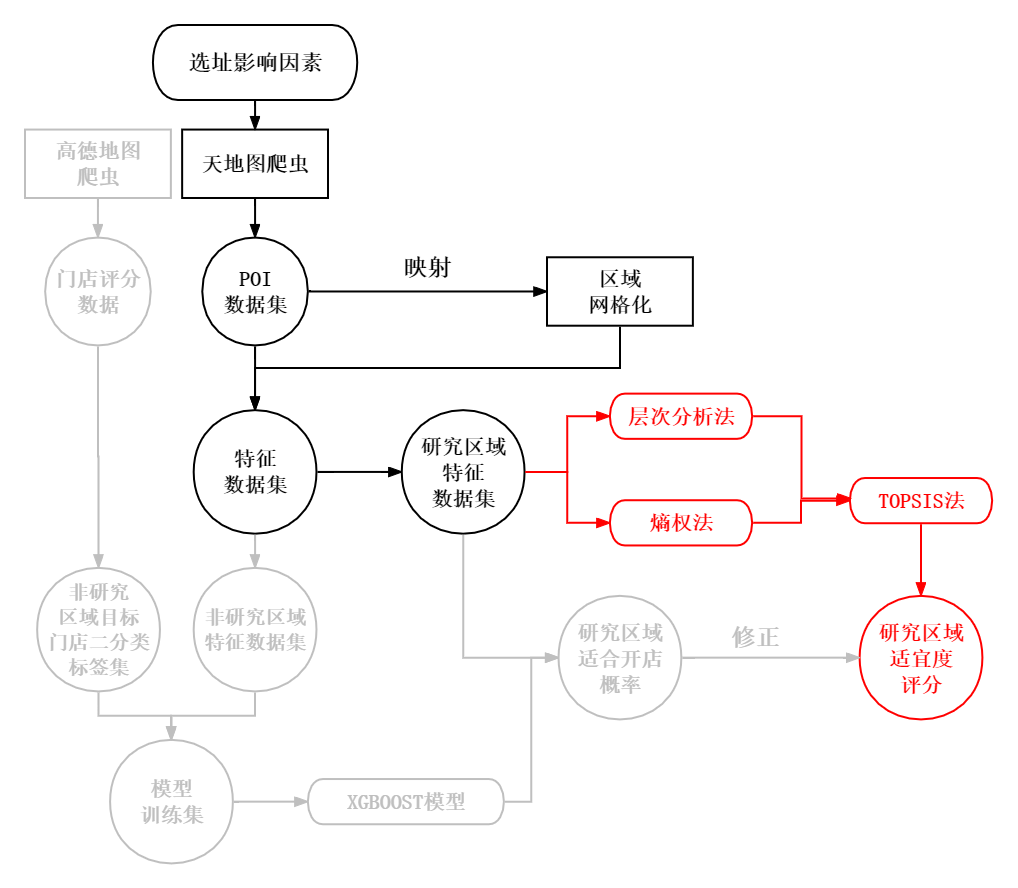
\includegraphics[width=1\textwidth]{pic/4.png}
      \end{minipage}
\end{frame}

\begin{frame}{研究思路}   
    \begin{minipage}{0.37\textwidth}
        % 左侧内容
        适宜度评分修正
        \begin{itemize}
            \item 修正原因
            \begin{itemize}
                \item 在评价类算法中,竞争强度被指定为负向指标
                \item 竞争强度具有两面性,适度竞争可吸引消费者,但过度竞争会导致恶性竞争,影响经济收益
    
            \end{itemize}
        \end{itemize}
  
      \end{minipage}
      \hfill
      \begin{minipage}{0.6\textwidth}
        % 插入图片
        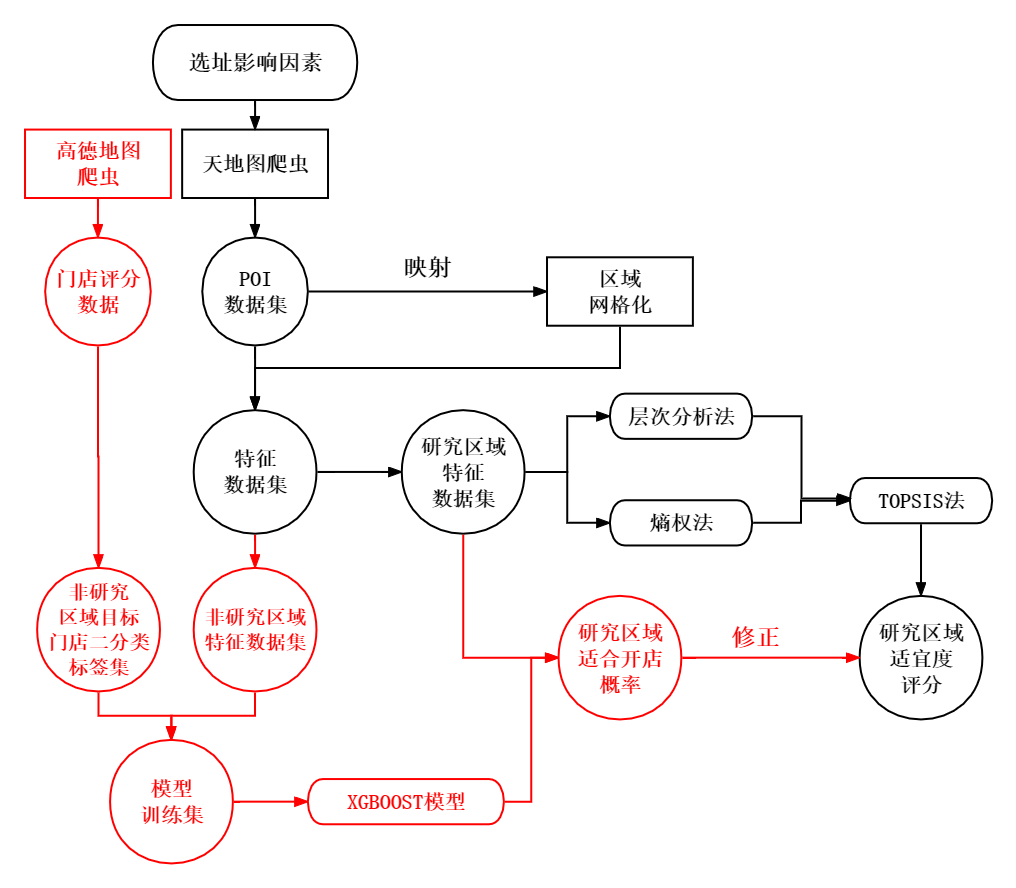
\includegraphics[width=1\textwidth]{pic/5.png}
      \end{minipage}
\end{frame}

\begin{frame}{研究思路}   
    \begin{minipage}{0.37\textwidth}
        % 左侧内容
        适宜度评分修正
        \begin{itemize}
            \item 修正步骤
            \begin{enumerate}
                \item 依据选址单元的高德地图门店评分值生成二分类标签集
                \item 利用非研究区域(广州市内,研究区域外)的数据集构建XGBOOST模型
                \item 利用模型预测研究区域的选址单元的适合开店概率对评分进行修正
    
            \end{enumerate}
        \end{itemize}
  
      \end{minipage}
      \hfill
      \begin{minipage}{0.6\textwidth}
        % 插入图片
        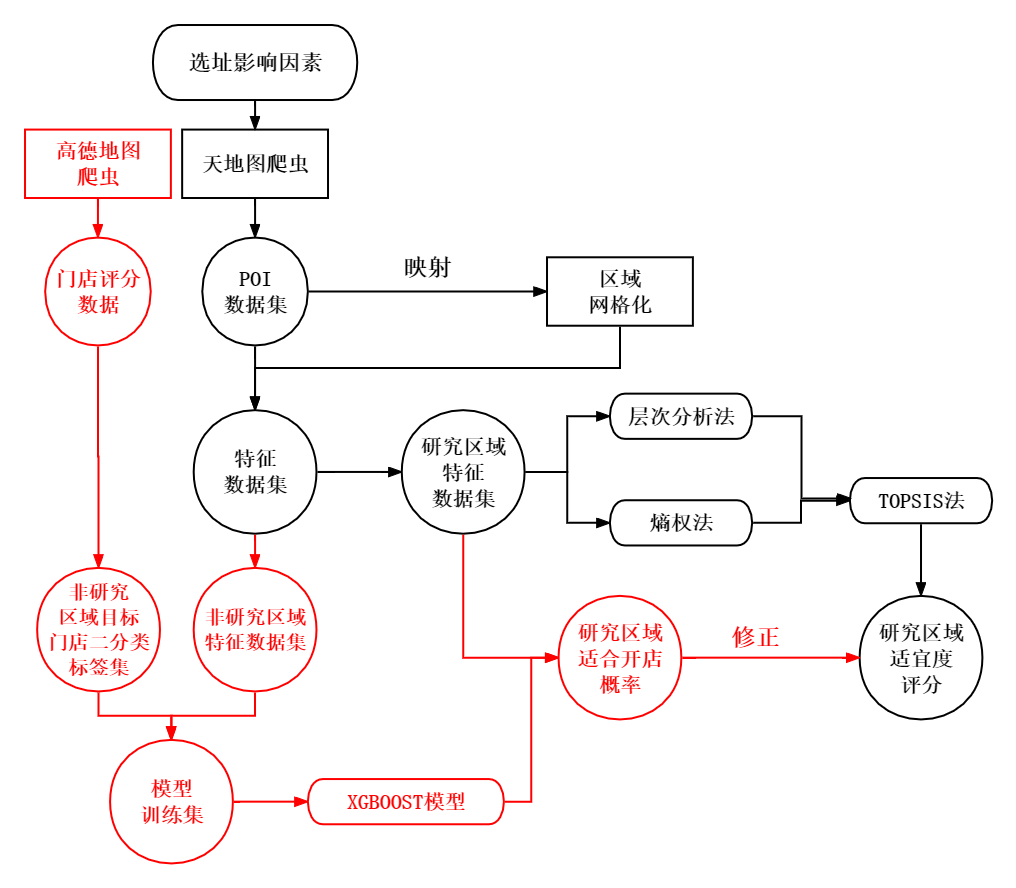
\includegraphics[width=1\textwidth]{pic/5.png}
      \end{minipage}
\end{frame}

\section{实验结果分析}
\begin{frame}{实验结果分析}
    \begin{minipage}{0.37\textwidth}
        % 左侧内容
        适宜度评分修正前后对比图{\footnotesize(颜色越深,适宜度评分越高)}
        \small
        \begin{itemize}
            \item 未修正的适宜度评分在冷饮店数量较多的区域较低,修正后有所提高,说明模型考虑了竞争的相对强度
            \item 适宜度评分较好的区域中都有目标选址的存在,表明模型很好地拟合了现有门店布局的空间特征
        \end{itemize}
  
      \end{minipage}
      \hfill
      \begin{minipage}{0.6\textwidth}
        % 插入图片
        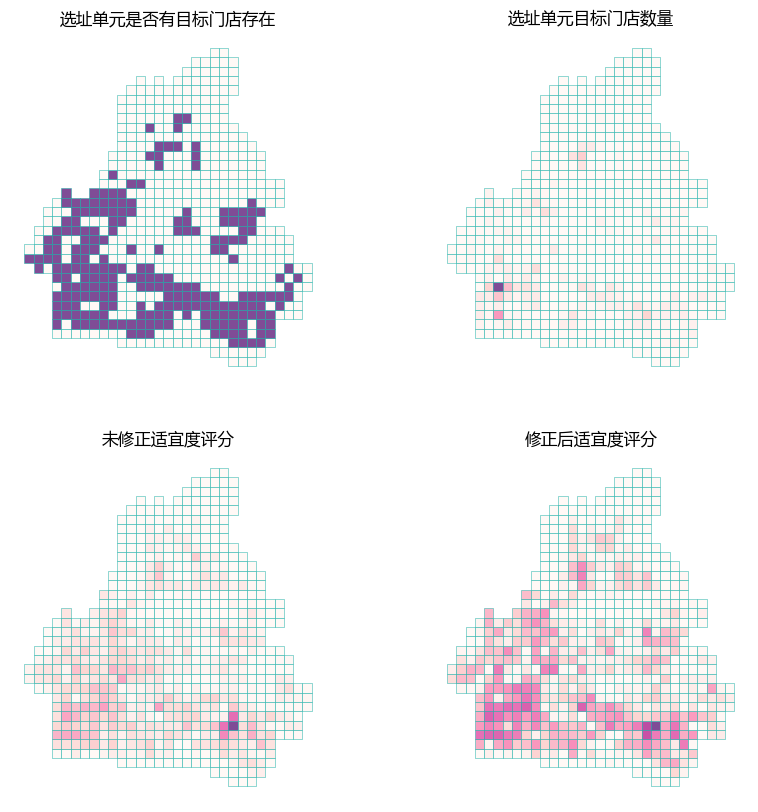
\includegraphics[width=1\textwidth]{pic/result1.png}
      \end{minipage}
\end{frame}

\begin{frame}{实验结果分析}
    \begin{minipage}{0.37\textwidth}
        % 左侧内容
        适宜度评分与天河区基础图层叠加图
        \small
        \begin{itemize}
            \item 冷饮店选址适宜度评分符合城市经济系统的“核心-边缘”理论
            \item 适宜度前五的区域集中在石牌、棠下、黄村街道。
            这些街道设施完善,交通发达,商业设施聚集,对冷饮店的发展有利。
        \end{itemize}
  
      \end{minipage}
      \hfill
      \begin{minipage}{0.6\textwidth}
        % 插入图片
        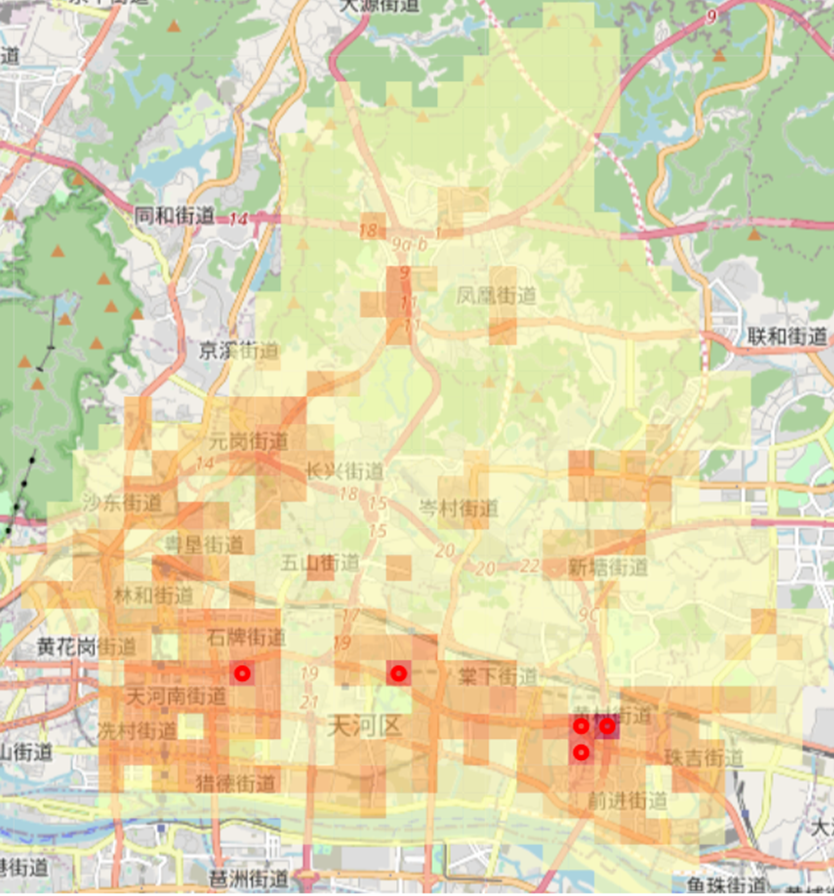
\includegraphics[width=1\textwidth]{pic/result2.png}
      \end{minipage}
\end{frame}


\begin{frame}{实验结果分析}
    \begin{minipage}{0.37\textwidth}
        % 左侧内容
        综上可得,选址模型能够较好地体现研究区域门店选址的适宜度与空间分布的异质性,可以为餐饮门店的选址提供决策依据。
      \end{minipage}
      \hfill
      \begin{minipage}{0.6\textwidth}
        % 插入图片
        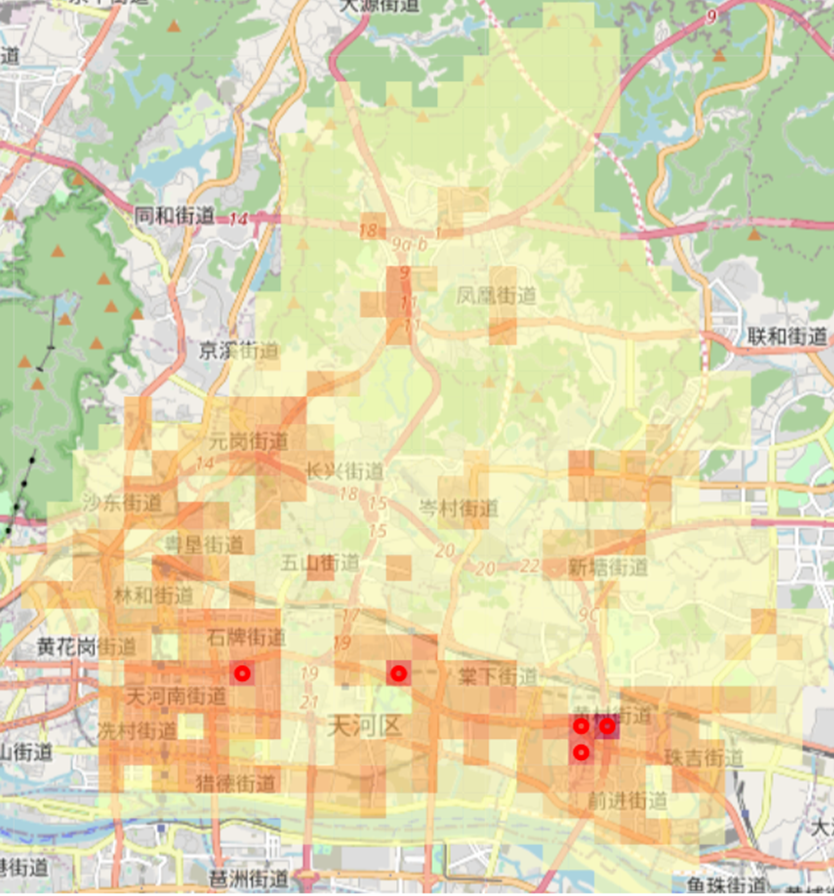
\includegraphics[width=1\textwidth]{pic/result2.png}
      \end{minipage}
\end{frame}



\section{总结与展望}
\begin{frame}{总结与展望}
    \begin{itemize}
        \item 论文创新点
        \begin{itemize}
            \item 本文的所有数据均来源自开源数据平台,数据可获取性较强
            \item 选址算法融合传统选址评价算法和机器学习算法,可以更加全面地对数据进行分析
        \end{itemize}
        \item 扩展方向
        \begin{itemize}
            \item 考虑更多的开源数据
            \item 考虑更多的指标,如空间统计量等
        \end{itemize}
    \end{itemize}
\end{frame}

\begin{frame}
    \begin{center}
        {\Large 谢谢观看}\\
        {\Large 请各位老师批评指正}
    \end{center}
\end{frame}


% \section{研究内容}

% \subsection{美化主题}

% \begin{frame}{这一份主题与原始的THU Beamer Theme区别在于}
%     \begin{itemize}
%         \item 顶栏的小点变成一行而不是多行
%         \item 中文采用楷书
%         \item 由于吉大校徽的配色有点艳丽,本文主题色采用了RGB\#336699,主题色可在JilinUniv.sty文件中修改
%         \item 更多该模板的功能可以参考 \url{https://www.latexstudio.net/archives/4051.html}
%     \end{itemize}
% \end{frame}

% \subsection{如何更好地做Beamer}

% \begin{frame}{Why Beamer}
%     \begin{itemize}
%         \item \LaTeX 广泛用于学术界,期刊会议论文模板
%     \end{itemize}
%     \begin{table}[h]
%         \centering
%         \begin{tabular}{c|c}
%             Microsoft\textsuperscript{\textregistered}  Word & \LaTeX \\
%             \hline
%             文字处理工具 & 专业排版软件 \\
%             容易上手,简单直观 & 容易上手 \\
%             所见即所得 & 所见即所想,所想即所得 \\
%             高级功能不易掌握 & 进阶难,但一般用不到 \\
%             处理长文档需要丰富经验 & 和短文档处理基本无异 \\
%             花费大量时间调格式 & 无需担心格式,专心作者内容 \\
%             公式排版差强人意 & 尤其擅长公式排版 \\
%             二进制格式,兼容性差 & 文本文件,易读、稳定 \\
%             付费商业许可 & 自由免费使用 \\
%         \end{tabular}
%     \end{table}
% \end{frame}

% \begin{frame}{排版举例}
%     \begin{exampleblock}{无编号公式} % 加 * 
%         \begin{equation*}
%             J(\theta) = \mathbb{E}_{\pi_\theta}[G_t] = \sum_{s\in\mathcal{S}} d^\pi (s)V^\pi(s)=\sum_{s\in\mathcal{S}} d^\pi(s)\sum_{a\in\mathcal{A}}\pi_\theta(a|s)Q^\pi(s,a)
%         \end{equation*}
%     \end{exampleblock}
%     \begin{exampleblock}{多行多列公式\footnote{如果公式中有文字出现,请用 $\backslash$mathrm\{\} 或者 $\backslash$text\{\} 包含,不然就会变成 $clip$,在公式里看起来比 $\mathrm{clip}$ 丑非常多。}}
%         % 使用 & 分隔
%         \begin{align}
%             Q_\mathrm{target}&=r+\gamma Q^\pi(s^\prime, \pi_\theta(s^\prime)+\epsilon)\\
%             \epsilon&\sim\mathrm{clip}(\mathcal{N}(0, \sigma), -c, c)\nonumber
%         \end{align}
%     \end{exampleblock}
% \end{frame}

% \begin{frame}
%     \begin{exampleblock}{编号多行公式}
%         % Taken from Mathmode.tex
%         \begin{multline}
%             A=\lim_{n\rightarrow\infty}\Delta x\left(a^{2}+\left(a^{2}+2a\Delta x+\left(\Delta x\right)^{2}\right)\right.\label{eq:reset}\\
%             +\left(a^{2}+2\cdot2a\Delta x+2^{2}\left(\Delta x\right)^{2}\right)\\
%             +\left(a^{2}+2\cdot3a\Delta x+3^{2}\left(\Delta x\right)^{2}\right)\\
%             +\ldots\\
%             \left.+\left(a^{2}+2\cdot(n-1)a\Delta x+(n-1)^{2}\left(\Delta x\right)^{2}\right)\right)\\
%             =\frac{1}{3}\left(b^{3}-a^{3}\right)
%         \end{multline}
%     \end{exampleblock}
% \end{frame}

% \begin{frame}{图形与分栏}
%     % From thuthesis user guide.
%     \begin{minipage}[c]{0.3\linewidth}
%         \psset{unit=0.8cm}
%         \begin{pspicture}(-1.75,-3)(3.25,4)
%             \psline[linewidth=0.25pt](0,0)(0,4)
%             \rput[tl]{0}(0.2,2){$\vec e_z$}
%             \rput[tr]{0}(-0.9,1.4){$\vec e$}
%             \rput[tl]{0}(2.8,-1.1){$\vec C_{ptm{ext}}$}
%             \rput[br]{0}(-0.3,2.1){$\theta$}
%             \rput{25}(0,0){%
%             \psframe[fillstyle=solid,fillcolor=lightgray,linewidth=.8pt](-0.1,-3.2)(0.1,0)}
%             \rput{25}(0,0){%
%             \psellipse[fillstyle=solid,fillcolor=yellow,linewidth=3pt](0,0)(1.5,0.5)}
%             \rput{25}(0,0){%
%             \psframe[fillstyle=solid,fillcolor=lightgray,linewidth=.8pt](-0.1,0)(0.1,3.2)}
%             \rput{25}(0,0){\psline[linecolor=red,linewidth=1.5pt]{->}(0,0)(0.,2)}
% %           \psRotation{0}(0,3.5){$\dot\phi$}
% %           \psRotation{25}(-1.2,2.6){$\dot\psi$}
%             \psline[linecolor=red,linewidth=1.25pt]{->}(0,0)(0,2)
%             \psline[linecolor=red,linewidth=1.25pt]{->}(0,0)(3,-1)
%             \psline[linecolor=red,linewidth=1.25pt]{->}(0,0)(2.85,-0.95)
%             \psarc{->}{2.1}{90}{112.5}
%             \rput[bl](.1,.01){C}
%         \end{pspicture}
%     \end{minipage}\hspace{1cm}
%     \begin{minipage}{0.5\linewidth}
%         \medskip
%         %\hspace{2cm}
%         \begin{figure}[h]
%             \centering
%             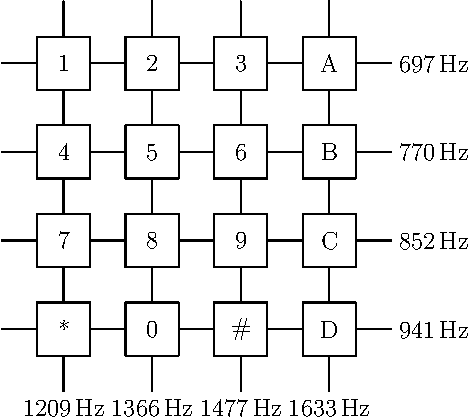
\includegraphics[height=.4\textheight]{pic/dtmf.pdf}
%         \end{figure}
%     \end{minipage}
% \end{frame}

% \begin{frame}[fragile]{\LaTeX{} 常用命令}
%     \begin{exampleblock}{命令}
%         \centering
%         \footnotesize
%         \begin{tabular}{llll}
%             \cmd{chapter} & \cmd{section} & \cmd{subsection} & \cmd{paragraph} \\
%             章 & 节 & 小节 & 带题头段落 \\\hline
%             \cmd{centering} & \cmd{emph} & \cmd{verb} & \cmd{url} \\
%             居中对齐 & 强调 & 原样输出 & 超链接 \\\hline
%             \cmd{footnote} & \cmd{item} & \cmd{caption} & \cmd{includegraphics} \\
%             脚注 & 列表条目 & 标题 & 插入图片 \\\hline
%             \cmd{label} & \cmd{cite} & \cmd{ref} \\
%             标号 & 引用参考文献 & 引用图表公式等\\\hline
%         \end{tabular}
%     \end{exampleblock}
%     \begin{exampleblock}{环境}
%         \centering
%         \footnotesize
%         \begin{tabular}{lll}
%             \env{table} & \env{figure} & \env{equation}\\
%             表格 & 图片 & 公式 \\\hline
%             \env{itemize} & \env{enumerate} & \env{description}\\
%             无编号列表 & 编号列表 & 描述 \\\hline
%         \end{tabular}
%     \end{exampleblock}
% \end{frame}

% \begin{frame}[fragile]{\LaTeX{} 环境命令举例}
%     \begin{minipage}{0.5\linewidth}
% \begin{lstlisting}[language=TeX]
% \begin{itemize}
%   \item A \item B
%   \item C
%   \begin{itemize}
%     \item C-1
%   \end{itemize}
% \end{itemize}
% \end{lstlisting}
%     \end{minipage}\hspace{1cm}
%     \begin{minipage}{0.3\linewidth}
%         \begin{itemize}
%             \item A
%             \item B
%             \item C
%             \begin{itemize}
%                 \item C-1
%             \end{itemize}
%         \end{itemize}
%     \end{minipage}
%     \medskip
%     \pause
%     \begin{minipage}{0.5\linewidth}
% \begin{lstlisting}[language=TeX]
% \begin{enumerate}
%   \item 白山 \item 旭日
%   \item 黑水
%   \begin{itemize}
%     \item[n+e] 红太阳
%   \end{itemize}
% \end{enumerate}
% \end{lstlisting}
%     \end{minipage}\hspace{1cm}
%     \begin{minipage}{0.3\linewidth}
%         \begin{enumerate}
%             \item 白山
%             \item 旭日
%             \item 黑水
%             \begin{itemize}
%                 \item[n+e] 红太阳
%             \end{itemize}
%         \end{enumerate}
%     \end{minipage}
% \end{frame}

% \begin{frame}[fragile]{\LaTeX{} 数学公式}
%     \begin{columns}
%         \begin{column}{.55\textwidth}
% \begin{lstlisting}[language=TeX]
% $V = \frac{4}{3}\pi r^3$

% \[
%   V = \frac{4}{3}\pi r^3
% \]

% \begin{equation}
%   \label{eq:vsphere}
%   V = \frac{4}{3}\pi r^3
% \end{equation}
% \end{lstlisting}
%         \end{column}
%         \begin{column}{.4\textwidth}
%             $V = \frac{4}{3}\pi r^3$
%             \[
%                 V = \frac{4}{3}\pi r^3
%             \]
%             \begin{equation}
%                 \label{eq:vsphere}
%                 V = \frac{4}{3}\pi r^3
%             \end{equation}
%         \end{column}
%     \end{columns}
%     \begin{itemize}
%         \item 更多内容请看 \href{https://zh.wikipedia.org/wiki/Help:数学公式}{\color{purple}{这里}}
%     \end{itemize}
% \end{frame}

% \begin{frame}[fragile]
%     \begin{columns}
%         \column{.6\textwidth}
% \begin{lstlisting}[language=TeX]
%     \begin{table}[htbp]
%       \caption{编号与含义}
%       \label{tab:number}
%       \centering
%       \begin{tabular}{cl}
%         \toprule
%         编号 & 含义 \\
%         \midrule
%         1 & 4.0 \\
%         2 & 3.7 \\
%         \bottomrule
%       \end{tabular}
%     \end{table}
%     公式~(\ref{eq:vsphere}) 的
%     编号与含义请参见
%     表~\ref{tab:number}。
% \end{lstlisting}
%         \column{.4\textwidth}
%         \begin{table}[htpb]
%             \centering
%             \caption{编号与含义}
%             \label{tab:number}
%             \begin{tabular}{cl}\toprule
%                 编号 & 含义 \\\midrule
%                 1 & 4.0\\
%                 2 & 3.7\\\bottomrule
%             \end{tabular}
%         \end{table}
%         \normalsize 公式~(\ref{eq:vsphere})的编号与含义请参见表~\ref{tab:number}。
%     \end{columns}
% \end{frame}

% \begin{frame}{作图}
%     \begin{itemize}
%         \item 矢量图 eps, ps, pdf
%         \begin{itemize}
%             \item METAPOST, pstricks, pgf $\ldots$
%             \item Xfig, Dia, Visio, Inkscape $\ldots$
%             \item Matlab / Excel 等保存为 pdf
%         \end{itemize}
%         \item 标量图 png, jpg, tiff $\ldots$
%         \begin{itemize}
%             \item 提高清晰度,避免发虚
%             \item 应尽量避免使用
%         \end{itemize}
%     \end{itemize}
%     \begin{figure}[htpb]
%         \centering
%         
\includegraphics[width=0.1\linewidth]{pic/scnulogo.eps}
%         \caption{这个校徽就是矢量图}
%     \end{figure}
% \end{frame}

% \section{总结与展望}
% \begin{frame}
%     \begin{itemize}
%         \item 我是一只酸菜鱼
%         \item 又酸又菜又多余
%         \item 我是一只黄焖鸡
%         \item 又黄又焖又辣鸡
%     \end{itemize}
% \end{frame}

% \section{参考文献}

% \begin{frame}[allowframebreaks]
%     \bibliography{ref}
%     \bibliographystyle{alpha}
%     % 如果参考文献太多的话,可以像下面这样调整字体:
%     % \tiny\bibliographystyle{alpha}
% \end{frame}

% \begin{frame}
%     \begin{center}
%         {\Huge\calligra Thanks!}
%     \end{center}
% \end{frame}

\end{document}